%\documentstyle[a4,14pt,marginitemize,latin1]{oldarticle}
\documentclass[a4,14pt,latin1]{article}
%HEVEA\externalcsstrue
%HEVEA\loadcssfile{../hevea.css}
\usepackage{graphicx}
\usepackage{float}
\usepackage{hevea,ifthen}
\begin{document}
%HEVEA\newcommand{\index}[1]{}
\begin{latexonly}
\parindent 0em
\parskip \baselineskip %.5ex
\itemsep 0ex
\end{latexonly}
\newcommand{\sectionref}[1]{section~\ref{#1}}
\newcommand{\chapterref}[1]{chapter~\ref{#1}}
\newcommand{\Chapterref}[1]{Chapter~\ref{#1}}
\newcommand{\figureref}[1]{figure~\ref{#1}}
\newcommand{\RASMUS}{{\sc Xrasmus}}
\newcommand{\UCRASMUS}{{\tt xrasmus}}
\newcommand{\MODIFY}{{\sc Xmodify}}
\newcommand{\X}{{\sc X}}
\newcommand{\UNIX}{{\sc UNIX}}
\newcommand{\FIX}[1]{$\langle\langle$#1$\rangle\rangle$}
\newcommand{\SET}[1]{\{#1\}}
\newcommand{\NT}[1]{$\langle$#1$\rangle$}
\newcommand{\BUTTON}[1]{\fbox{\tt #1}}
\newcommand{\FBUTTON}[1]{\framebox[2em]{\rule[-.5ex]{0em}{2.5ex}{\tt #1}}}
\newcommand{\META}[1]{{\rm\bf #1}\index{syntaks!#1}}
\newcommand{\METAPLUS}[1]{{\rm\bf #1}$^{\displaystyle +}$\index{syntaks!#1}}
\newcommand{\METASTAR}[1]{{\rm\bf #1}$^{\displaystyle \,*}$\index{syntaks!#1}}
\newcommand{\METAPLUSLIST}[1]{{\rm\bf #1}$^{\displaystyle
                                            \,+\lambda}$\index{syntaks!#1}}
\newcommand{\METASTARLIST}[1]{{\rm\bf #1}$^{\displaystyle
                                            \,*\lambda}$\index{syntaks!#1}}
\newcommand{\METAOPT}[1]{{\rm\bf #1}$^{\displaystyle
                                            \,\circ}$\index{syntaks!#1}}
\newcommand{\IS}{$::=\;\;\;$}
\newcommand{\OR}{$\;\;\mid\;\;$}
%
\newcommand{\define}[1]{{\it #1\/}}
\newcommand{\RAS}{{\sc Rasmus}}
\newcommand{\EMACS}{{\sc Emacs}}
\newcommand{\menu}[1]{\fbox{\fbox{\tt #1}}}
\newcommand{\mopt}[1]{\fbox{\tt #1}}
%
\pagenumbering{roman}
\begin{latexonly}
  \tableofcontents
  \newpage
\end{latexonly}
\pagenumbering{arabic}
%\section{Introduction}
This manual describes how to use the \RAS{} system together with the
\EMACS{} editor. It also describes how to obtain {\it persistence\/},
i.e. how to save results between sessions. Finally, it describes what
\RAS{} expressions look like, and what they mean. Basic familiarity
with \EMACS{} is assumed, cf. the {\sc Trine} manual.

\section{The Interpreter}
\label{theinterpreter}
The purpose of the \RAS{} interpreter is to evaluate expressions typed
by the user.   This chapter, describes the \RAS{} interpreter.

\subsection{Getting started}
\label{thewindowsystem}
To start \RAS{} from within \EMACS{}, use the \menu{Modes} menu. It has
two entries relating to \RAS{}:
\begin{itemize}
\bf
\item Rasmus
\item Rasmus...
\end{itemize}
The first entry will open up a new frame called {\tt RASMUS}, for the
communication with the \RAS{} interpreter. The second entry will start
by prompting for directories, before opening up the new frame, but is
otherwise identical to the first. The second entry will be further
explained in \chapterref{persistence}.

\samepage The \RAS{} frame contains a new menu, \menu{Rasmus} menu.
Its content looks something like \figureref{fig:rasmus-menu}.
%\begin{figure}[p]
\begin{figure}[H]
  \begin{center} \tt
    \begin{tabular}{|l|}
      \hline
      Evaluate\\
      Save last... \\
      Change name...\\
      Clean \\
      Modify\\
      Quit \\ 
      \hline
    \end{tabular}
  \end{center}
  \caption{The \menu{Rasmus} menu.}
  \label{fig:rasmus-menu}
\end{figure}
The explanation of \mopt{Evaluate} is described in the following,
while the explanation of \mopt{Save last...}~, \mopt{Change name...}
and \mopt{Clean} are deferred to \chapterref{persistence}. The
\mopt{Modify} entry will be described in a separate note.

\subsection{Getting along}
The \RAS{} frame consists of two separate parts (cf.
\figureref{initialinterpreter}). These parts are in the terminology of
\EMACS{} called \define{windows} (not to be confused with X-windows).
Each window has its own status-line. The top window is called the
\define{output} window, or the \define{passive} part. The bottom
window is called the \define{input} window or the \define{active}
part. Input to the interpreter is typed into the active window, and
the interpreter will respond in the passive window.
%\begin{figure}[h!p]
\begin{figure}[H]
%\centerline{\psfig{figure=rasfig-initial.ps}}
\centerline{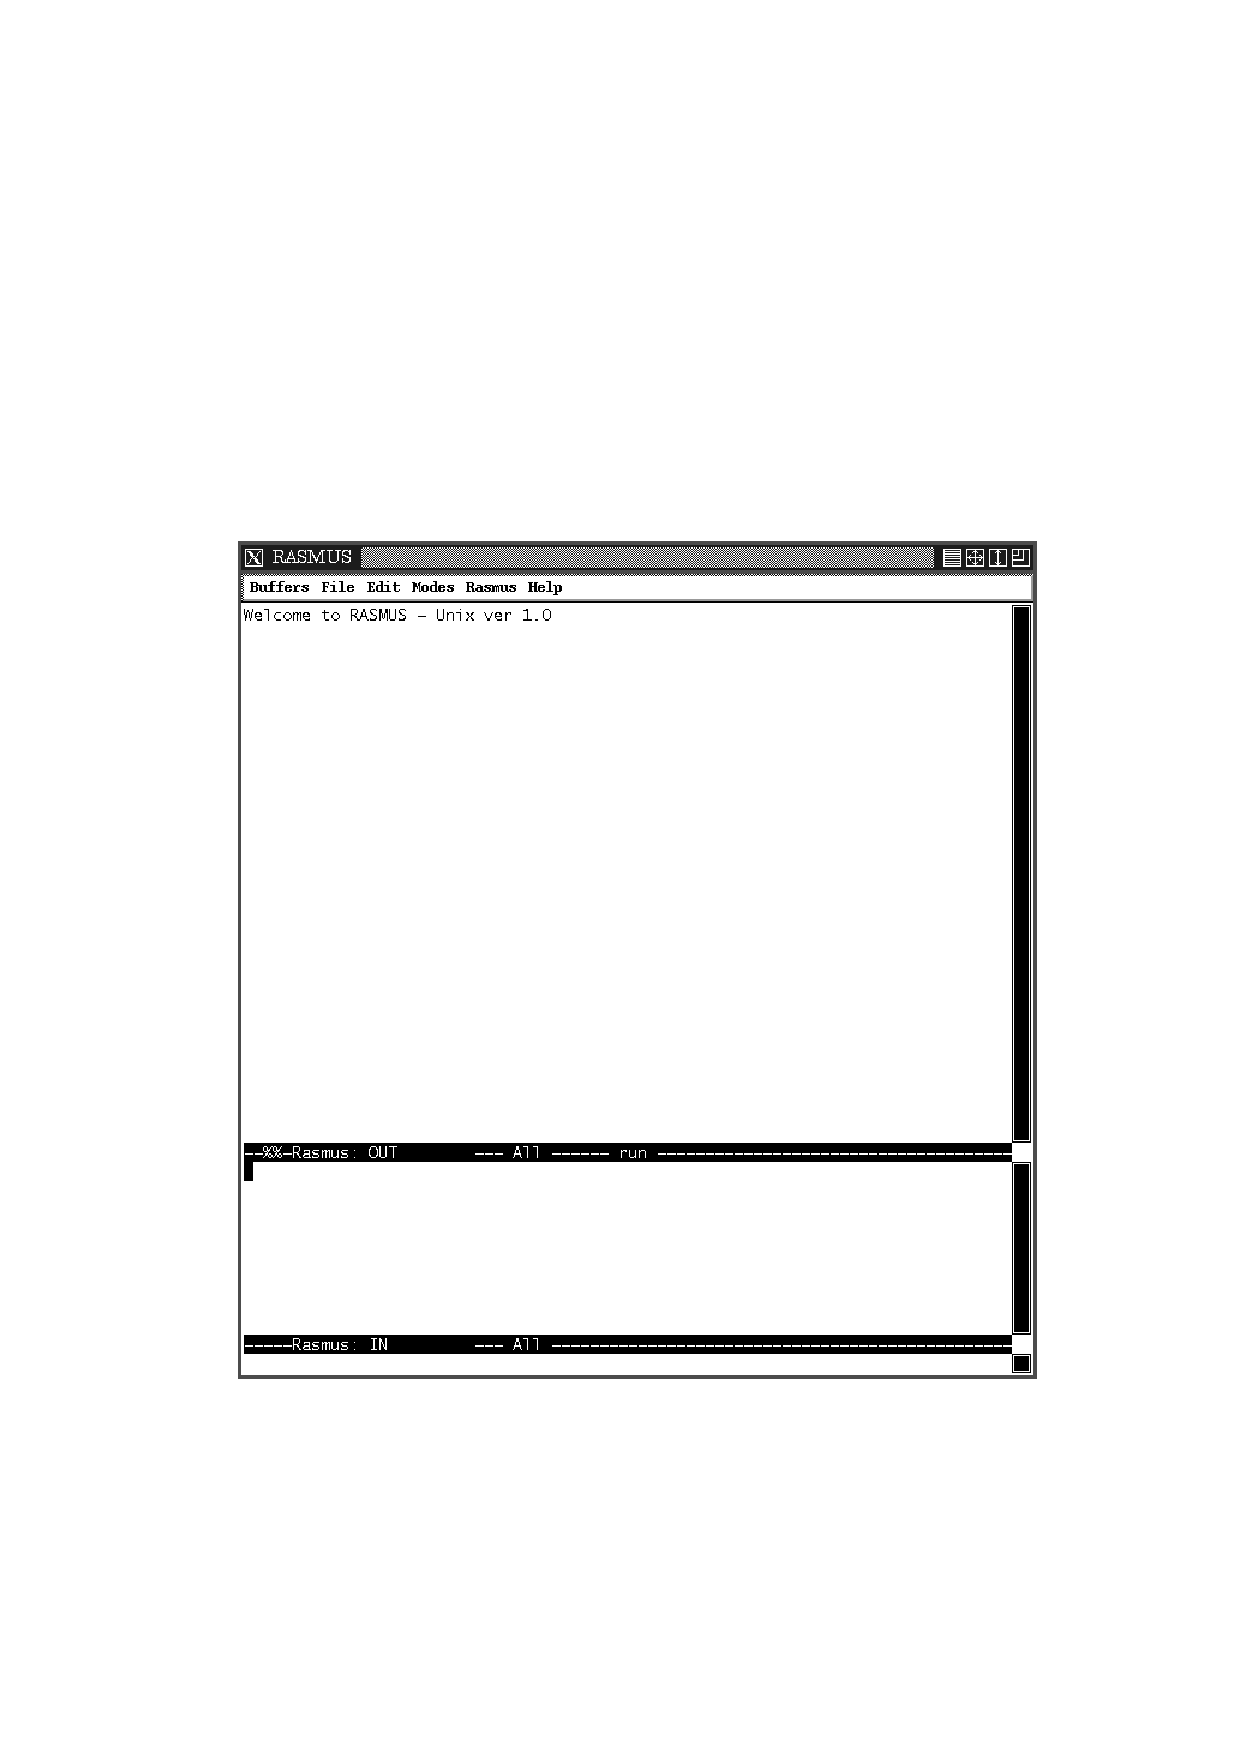
\includegraphics[]{rasfig-initial.pdf}}
\caption{Initial appearance of interpreter.}
\label{initialinterpreter}
\end{figure}

In fact, the active and passive windows are ordinary \EMACS{} buffers,
which operate in a special \RAS{} major mode. This means that anything
you can do with a buffer, you can also do with the \RAS{} windows,
including printing and saving.

In order to type in an expression for the interpreter to evaluate, the
input buffer must be made active. This is done either via the {\tt
  Buffers} menu, or by placing the cursor in the input window and
pressing the left mousebutton (you may also place the cursor in the
passive window, but the system will not allow you to alter the buffer
it displays).

Suppose you have typed in the following expression:
\begin{center}
\parbox{10em}{\tt
1+2+3+4+5+6+\\
7+8+9+10}
\end{center}
Your \RAS{} frame will now look as in \figureref{anexpininterpreter}.
\begin{figure}[p]
%\centerline{\psfig{figure=rasfig-firstexp.ps}}
\centerline{\includegraphics[]{rasfig-firstexp.pdf}}
\caption{Typing the first expression.}
\label{anexpininterpreter}
\end{figure}
In order to have the interpreter evaluate the expression, you must use
the \menu{Rasmus} menu. If you select \mopt{Evaluate}, your frame will
end up looking like \figureref{oneexpevaluated}.
\begin{figure}[p]
%\centerline{\psfig{figure=rasfig-firsteval.ps}}
\centerline{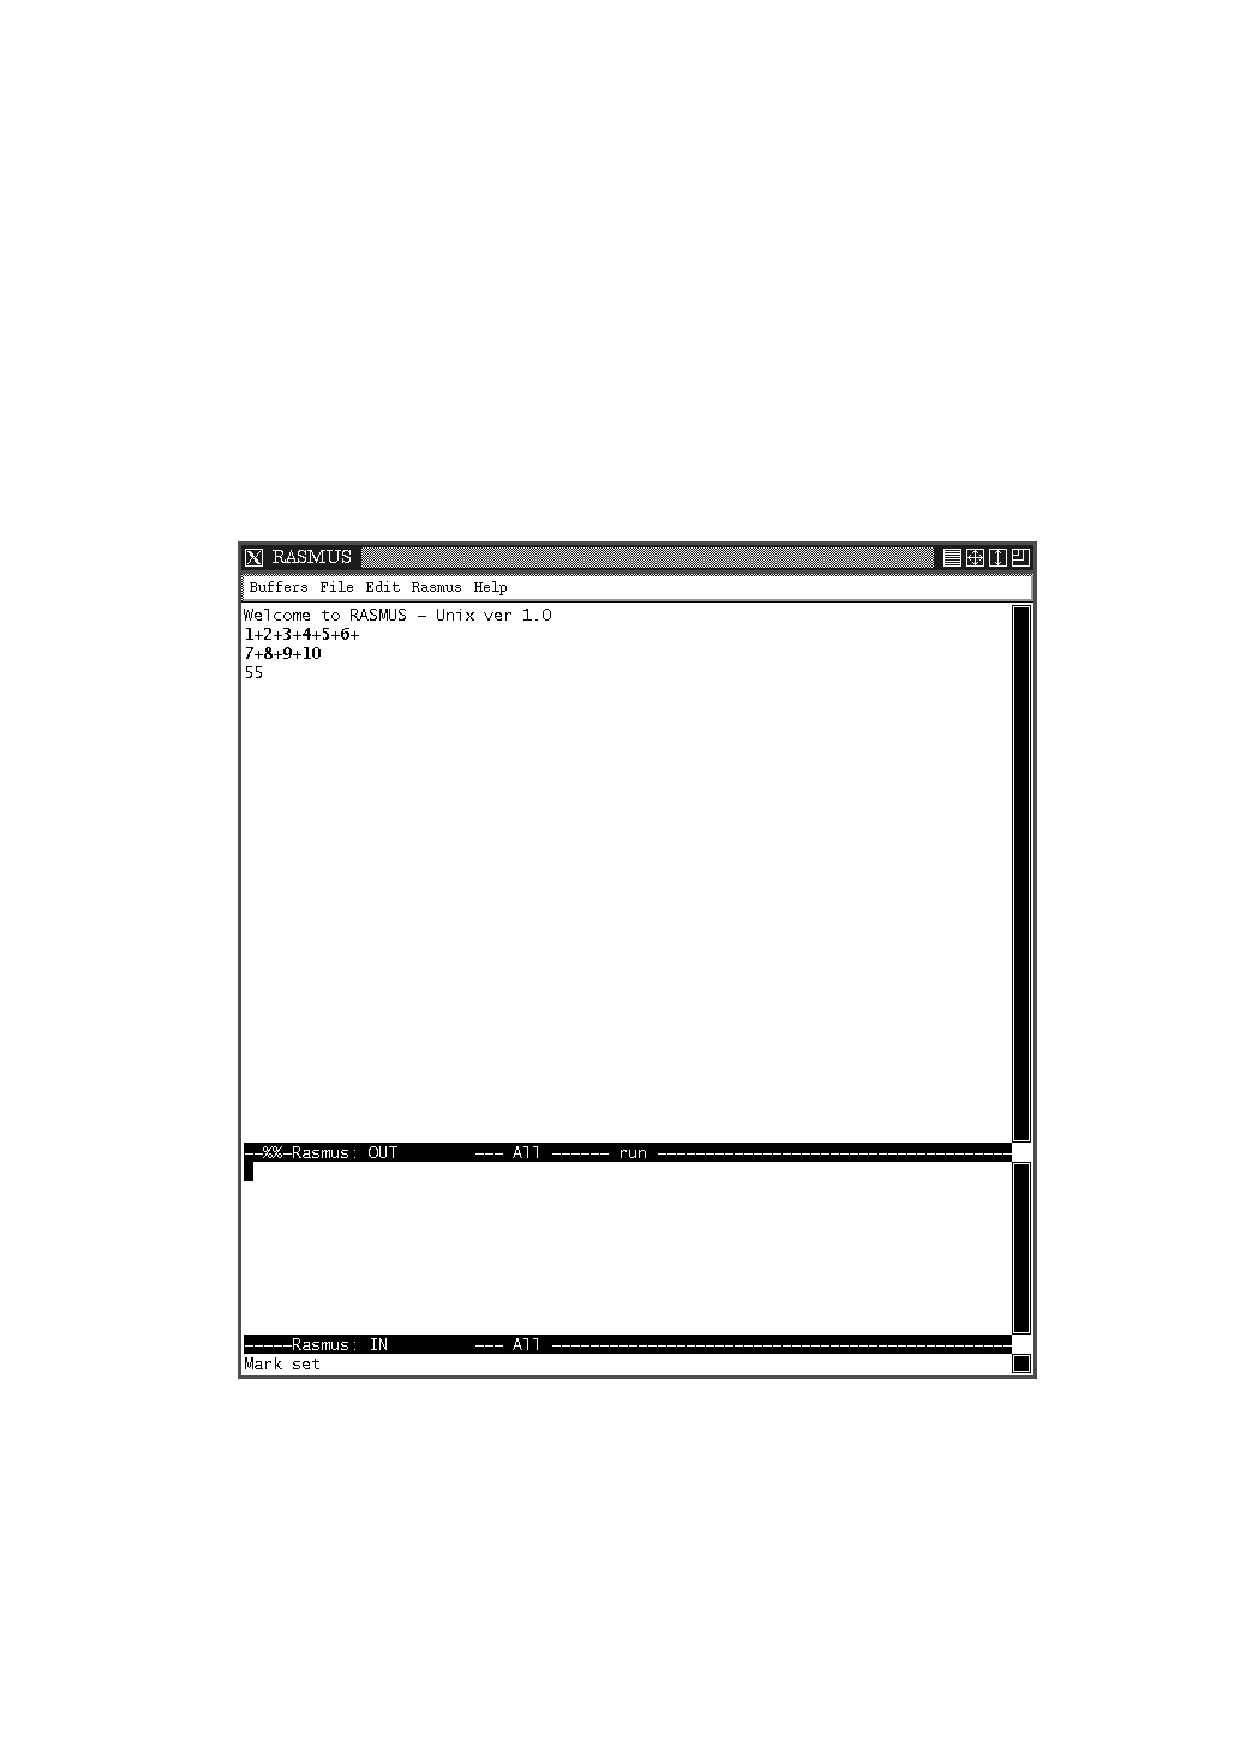
\includegraphics[]{rasfig-firsteval.pdf}}
\caption{After the evaluation.}
\label{oneexpevaluated}
\end{figure}
The expression has been copied from the active window into the passive,
using a different font, so that you may distinguish your input from
the output of the interpreter. The interpreter evaluates the
expression, and inserts the result into the output buffer. The active
window is then cleared.

If you have typed in an illegal expression, the active part is not
cleared, which means that you can edit the expression. What constitutes legal
expressions is further described in \chapterref{expressions}.

To get rid of the interpreter, you can use the \mopt{Quit} entry of the
\menu{Rasmus} menu. This will delete the {\tt RASMUS} frame and the
corresponding input and output buffers.

\section{Introduction}

This manual describes how to use the Rasmus system. It also describes
how to obtain persistence, i.e. how to save results between
sessions. Finally, it describes what Rasmus expressions look like, and
what they mean.

\section{The Interpreter}

The purpose of the Rasmus interpreter is to evaluate expressions typed
by the user. This chapter describes the \RAS{} interpreter.

\subsection{Getting started}

To start \RAS{} execute the \mopt{rasmus} file. This opens a graphical
user interface (GUI) window similar to the one shown in
\figureref{fig:initial_window}.

\begin{figure}
  \centering
  \ifthenelse{\boolean{hevea}}{
    \imgsrc{initial_window.png}
  }{
    \includegraphics[scale=0.5]{initial_window.png}
  }
  \caption{The initial \RAS{} window}
  \label{fig:initial_window}
\end{figure}

In the following we describe how to evaluate \RAS{} expressions in the
interpreter. Next we walk through the features that are available in
the GUI.

\subsection{Getting along}

On the left side of the main window there is a {\it
  Read-Eval-Print-Loop} (REPL) interpreter where \RAS{} expressions
can be typed and evaluated. The left side will be refered to as the
{\it interpreter}. On the right side we see a list of names and
values. The names are the variables that currently exist in the global
scope and the values are the corresponding values. If a variable's
value is {\it Relation} then it is possible to inspect that relation
by double clicking the variable name. This will pop up a new window
similar to the one in \figureref{fig:relation_view}.

\begin{figure}
  \centering
  \ifthenelse{\boolean{hevea}}{
    \imgsrc{relation_view.png}
  }{
    \includegraphics[scale=0.5]{relation_view.png}
  }
  \caption{Inspecting the relation \mopt{Kampe}}{Insepecting the relation \mopt{Kampe}. Note that the
    relation cannot be modified here, that is only possible through
    interaction with the \RAS{} interpreter. It is however possible to
    sort the tuples by clicking on the header. Note that it is a
    stable sort, so you can sort the tuples breaking ties properly.}
  \label{fig:relation_view}
\end{figure}

Typing in expressions in the interpreter and pressing return makes the
interpreter evaluate the expression. Suppose you have typed in the
following expression:

\begin{center}
{\tt x := 1+2+3+4+5+6+\\
7+8+9+10}
\end{center}

Your \RAS{} window will now look as in \figureref{fig:first_exp}. Note
that due to the last ``+'' on the first line the interpreter was still
waiting for input. Had the ``+'' been omitted the first line would
have been evaluated before the second line could be typed in the
interpreter. Furthermore, observe that a new name appeared in the
environment list on the right. This happened because a new variable,
\mopt{x}, has been defined.

\begin{figure}
  \centering
  \ifthenelse{\boolean{hevea}}{
    \imgsrc{first_exp.png}
  }{
    \includegraphics[scale=0.5]{first_exp.png}
  }
  \caption{The first \RAS{} expression.}
  \label{fig:first_exp}
\end{figure}


If you type an illegal expression, the \RAS{} interpreter will do its
best to diagnose the error and provide a useful error message, such
that you can correct the error. What constitutes a legal expression is
further described in \Chapterref{expressions}.

To close the \RAS{} system go to \menu{File} and \mopt{Quit}.

\subsection{The Editor}

Often we want to produce more complicated pieces of code rather than
simple expressions. To accomodate this the \RAS{} system contains a
development environment as well. To open a new file in the editor go
to \menu{File} and then click \mopt{New}. This opens an editor where
\RAS{} code can be written. Note that there is simple syntax
highlighting and intellisense (i.e.\ a red lines appear under invalid
expressions). Once you have written your code you can send it to the
interpreter by either going to \menu{File} and click \mopt{Run}, or by
using the shortcut Ctrl+R.

The code you type can be saved in \RAS{} code files by using
\menu{File}, \mopt{Save}. As a side note, \RAS{} code files have the
extension ``.rm'' . If you want to load previously written \RAS{} code
files you have to use the \menu{File} menu in the main window followed
by clicking \mopt{Open} and locating the file on your system.


\subsection{Preferences and Help}

It is possible to do some configuration of your \RAS{} system, such as
changing font types and colors. Going to \menu{Edit} and
\mopt{Preferences} opens a dialog where you can change these visual
features. An important setting is the \mopt{Environment Path}. This is
the directory where all relations are stored and also where they are
automatically loaded from when \RAS{} is started. It is recommended
that you use the \mopt{Environment Path} as workspace but you remember
to export relations to other places as well. Further information on
how relations are stored and retrieved can be found in
\sectionref{persistence}.

In the \menu{Help} menu you can find a tutorial on \RAS{} and the
\RAS{} manual (this document).

%\newpage
\section{Persistence}
\label{persistence}
One of the primary differences between an ordinary programming
language and a database language is that the latter works on
persistent data, i.e., we want to be able to start a session with the
data we had when we ended the last session.  We discuss this further
in \sectionref{startendsession}.  Another difference is that a
database should be able to deal with huge amounts of external data. In
particular, a database language is required to include a specification
of how external data can be read by the system. This is the subject of
\sectionref{exrelformat} and \sectionref{exrelcsvformat}.

\subsection{Starting and Ending a Session}
\label{startendsession}
As described in the beginning, \RAS{} is started executing the 
\mopt{rasmus} file.

When starting a session, \RAS{} reads the \mopt{Environment Path} as
set in \menu{Edit}, \mopt{Preferences} and establishes the relations
represented by the directory. These relations are the files in that
directory with the ``rdb'' file extension.

As an example, suppose we have started \RAS{} with the
\mopt{Environment Path} pointing to a directory where there is a
relation called {\tt children}.  After starting up the relation {\tt
  children} is loaded and can be seen in the environment (\figureref{fig:startup}).

\begin{figure}[bp]
  \centering
  \ifthenelse{\boolean{hevea}}{
    \imgsrc{persistence_startup.png}
  }{
    \includegraphics[scale=0.5]{persistence_startup.png}
  }
  \caption{Starting up.}
  \label{fig:startup}
\end{figure}

%% \begin{figure}[bp]
%% %\centerline{\psfig{figure=rasfig-tinyload.ps}}
%% \centerline{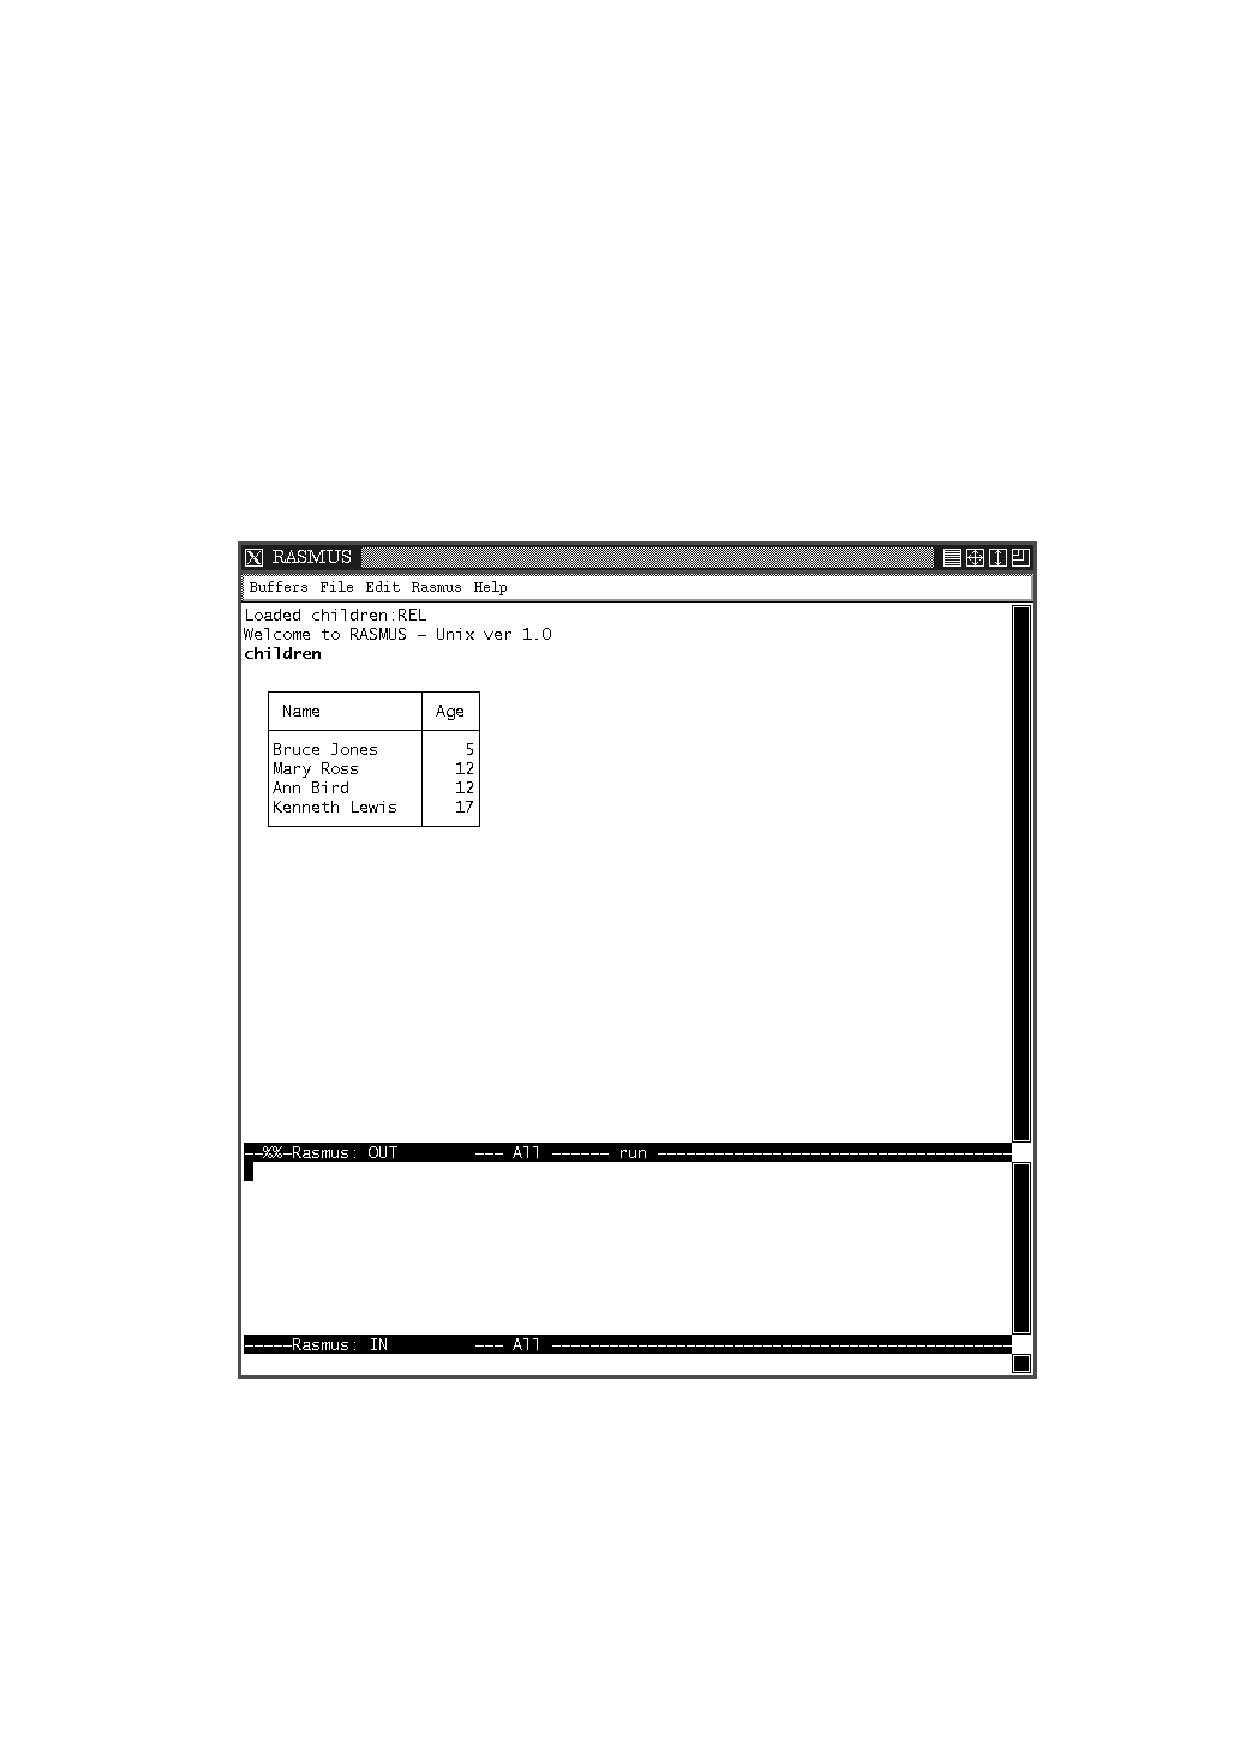
\includegraphics[]{rasfig-tinyload.pdf}}
%% \caption{A small relation.}
%% \label{tinyload}
%% \end{figure}

Double clicking the {\tt children} relation in the environment list
brings up the {\it relation view} (\figureref{fig:relation_view}). If
you want to export a relation from the \RAS{} system, go to
\menu{File} in the relation view and click \mopt{Export CSV}. This
brings up a dialog where you can decide where to save the file on your
disk.

\begin{figure}
  \centering
  \ifthenelse{\boolean{hevea}}{
    \imgsrc{children_relation.png}
  }{
    \includegraphics[scale=0.5]{children_relation.png}
  }
  \caption{Relation view of the example relation {\tt children}.}
  \label{fig:child_relation}
\end{figure}

It is also possible to save (copy) relations under a different name by
clicking the \mopt{Save as global} item in the \menu{File} menu.

If you want to save the result of an earlier evaluated expression, you
must reevaluate it and assign it to a variable using the \RAS{}
assignment syntax in the interpreter. Remember that the expression is
listed somewhere in the interpreter's history, and using the up and
down arrow keys on your keyboard you go through the history of
evaluated expressions.

Deleting a relation from the environment is achieved through the
\menu{File} menu in the main window and clicking \mopt{Delete
  relation}. This brings up a dialog asking for the name of the
relation to delete. Suppose we had made a copy of the {\tt children}
relation by the name of {\tt youngpeople} and we wanted to delete
it. Going through the two steps would bring us to the dialog seen in
\figureref{fig:delete_relation}. Clicking ``Ok'' removes {\tt
  YoungPeople} from the environment and it deletes the corresponding
relation file in the \mopt{Environment Path}.

\begin{quote}
  \bf Note that a relation is irretrieveably lost when it is deleted.
\end{quote}

\begin{figure}[bp]
  \centering
  \ifthenelse{\boolean{hevea}}{
    \imgsrc{delete_relation.png}
  }{
    \includegraphics[scale=0.5]{delete_relation.png}
  }
  \caption{Deleting a relation.}
  \label{fig:delete_relation}
\end{figure}

\subsection{External Relation Format}
\label{exrelformat}
Sometimes data is produced by other programs or have been collected by
people over time and the question naturally arises: how can such data
be read into a relation {\em automatically}? For this purpose, we
describe the {\em external relation format}. This is the format in
which relations are kept in the directories. So, obviously, if we can
transform data to this format (automatically), then this data can be
read into the system.

A relation in external format looks as illustrated in
\figureref{relformat}.
\begin{figure}[hp]
  \begin{center}
    \begin{tabular}{l}
      \NT{number of attribute names} \\
      \NT{type} \NT{name} \\
      \hspace*{1em}$\cdot$ \\
      \hspace*{1em}$\cdot$ \\
      \NT{type} \NT{name} \\
      \NT{field} \\
      \hspace*{1em}$\cdot$ \\
      \hspace*{1em}$\cdot$ \\
      \NT{field}
    \end{tabular}
  \end{center}
  \caption{External relation format.}
  \label{relformat}
\end{figure}
Here, \NT{type} can be either T, I, or B, representing the three
atomic types {\sc Text}, {\sc Integer} and {\sc Boolean}.

The external format of the {\tt children} relation would be as
depicted in \figureref{tinyformat}.
\begin{figure}[hp]
  \begin{center}
    \begin{tabular}{l}
      $2$ \\
      T Name \\
      I Age \\
      Bruce Jones \\
      5 \\
      Mary Ross \\
      12 \\
      Ann Bird \\
      12 \\
      Kenneth Lewis \\
      17
    \end{tabular}
  \end{center}
  \caption{External relation format of the {\tt children} relation.}
  \label{tinyformat}
\end{figure}

Relations are stored in external format as ordinary text files.  The
text file is named after the relation name, by adding an extension of
{\tt .rdb}. So our example relation was stored in a file {\tt
  children.rdb} with the exact contents of \figureref{tinyformat}.
This file can be loaded into \RAS{} by storing it in the
\mopt{Environment Path}.

\subsection{Working with CSV Files}
\label{exrelcsvformat}
Today much data is stored in CSV (Comma Seperated Value) files, and
\RAS{} is capable of reading and writing relations from and to CSV
files. Here we describe how \RAS{} interprets a CSV file when it is
loaded.

A CSV files consists of zero or more lines. Each line contains the
same number of fields seperated commas (,). A field may be enclosed by
quotes ("\textless content\textgreater "). Let $m$ be the number of
fields and $n$ be the number of rows, then the content of the first
field of the first row is $f_{1,1}$, and the content of the very last
field is $f_{n,m}$.

When reading a CSV file \RAS{} tries to guess the type of each
attribute in the tuples of the relation. This is done by guessing the
type of each attribute in turn. The type of the first attribute is
inferred based on the content of the fields $f_{2,1}, f_{3,1},\ldots,
f_{n, 1}$. In general the $j$th attribute's type is guessed based on
the contents of $f_{2, j}, f_{3, j},\ldots, f_{n, j}$. The type of an
attribute is guessed as follows. If all the fields contain an integer,
the type is {\sc Int}. If all the fields contain either {\tt true} or
{\tt false}, the type is {\sc Boolean}. Otherwise the type is {\sc Text}.

Note the first line of fields have been ignored. This is because it
might be the names of the attributes (also known as the \emph{header}
of the column). If all fields $f_{i,j}$ for $1 \le i \le n$ and $1 \le
j \le m$ are textual fields, then the first row is interpreted as
values rather than as the names of the attributes. In this case the
names of the columns are {\tt column0}, {\tt column1}, etc. Otherwise
the field $f_{1,j}$ for $1 \le j \le m$ is interpreted as the name of
column $j$.

A relation in CSV format looks as illustrated in
\figureref{csvformat}.
\begin{figure}[hp]
  \begin{center}
    \begin{tabular}{l}
      \NT{$f_{1,1}$},\NT{$f_{1,2}$}, $\ldots$ ,\NT{$f_{1,m}$} \\
      \NT{$f_{2,1}$},\NT{$f_{2,2}$}, $\ldots$ ,\NT{$f_{2,m}$} \\
      \hspace*{1em}$\cdot$ \\
      \hspace*{1em}$\cdot$ \\
      \NT{$f_{n,1}$},\NT{$f_{n,2}$}, $\ldots$ ,\NT{$f_{n,m}$} \\
    \end{tabular}
  \end{center}
  \caption{External CSV format.}
  \label{csvformat}
\end{figure}

%% The special case where the CSV file has zero lines is interpreted as
%% the {\tt zero} relation.

The CSV file of the {\tt children} relation would be as depicted in
\figureref{childrencsv}. Looking through \figureref{childrencsv}, we
see \RAS{} can infer that the type of the {\tt Age} column is {\sc
  Int}, since all values except the first value in that column are
integers.

\begin{figure}[hp]
  \begin{center}
    \begin{tabular}{l}
      Name,Age\\
      Bruce Jones,5\\
      Mary Rose,12\\
      Ann Bird,12\\
      Kenneth Lewis,17
    \end{tabular}
  \end{center}
  \caption{The {\tt children} relation as a CSV file.}
  \label{childrencsv}
\end{figure}


\clearpage
\section{Expressions}
\label{expressions}
In this chapter, we define the set of \RAS{} expressions. We do this
in several steps. First, we give a grammar from which expressions must
be generated. Afterwards, we give an informal semantics of \RAS{}
expressions.  In connection with this semantics, we restrict the set
of expressions further by adding type constraints.

\subsection{Grammar}
In the following, we define some notation:
\begin{itemize}
\item {\bf Category}$^{\displaystyle \,*}$ is a sequence of {\bf Category}
\item {\bf Category}$^{\displaystyle +}$ is a nonempty sequence of
                                                            {\bf Category}
\item {\bf Category}$^{\displaystyle \,*\lambda}$ is a comma separated sequence
                                                         of {\bf Category}
\item {\bf Category}$^{\displaystyle +\lambda}$ is a nonempty comma separated
                                                sequence of {\bf Category}
\item {\bf Category}$^{\displaystyle \circ}$ is either 0 or 1 of
                                                            {\bf Category}
\end{itemize}
In the following, a grammar for \RAS{} expressions is presented.

{\tt
\begin{tabbing}
\hspace*{4cm}\=\IS\=\hspace*{1cm}\=\kill
\META{Exp}\>\IS\>\META{AtomConst}\OR \\
          \>   \>\META{RelConst}\OR \\
          \>   \>\META{StandardConst}\OR \\
          \>   \>tup ( \METASTARLIST{NameExp} )\OR \\
          \>   \>rel ( \META{Exp} )\OR \\
          \>   \>func ( \METASTARLIST{NameType} ) -> ( \META{Type} ) \\
          \>   \> \>\META{Exp} \\
          \>   \>end\OR \\
          \>   \>\META{Name}\OR \\
          \>   \>\META{Name} := \META{Exp}\OR \\
          \>   \>\#\OR \\
          \>   \>@ ( \META{Exp} )\OR \\
          \>   \>not \META{Exp}\OR \\
          \>   \>\META{Exp} and \META{Exp}\OR \\
          \>   \>\META{Exp} or \META{Exp}\OR \\
          \>   \>- \META{Exp}\OR \\
          \>   \>\META{Exp} + \META{Exp}\OR \\
          \>   \>\META{Exp} - \META{Exp}\OR \\
          \>   \>\META{Exp} * \META{Exp}\OR \\
          \>   \>\META{Exp} / \META{Exp}\OR \\
          \>   \>\META{Exp} mod \META{Exp}\OR \\
          \>   \>\META{Exp} ++ \META{Exp}\OR \\
          \>   \>\META{Exp} ; \META{Exp}\OR \\
          \>   \>| \META{Exp} |\OR \\
          \>   \>\META{Exp} << \META{Exp}\OR \\
          \>   \>\META{Exp} .\ \META{Name}\OR \\
          \>   \>\META{Exp} \verb"\" \META{Name}\OR \\
          \>   \>has ( \META{Exp} , \META{Name} )\OR \\
          \>   \>\META{Exp} \META{ProjSym} \METAPLUSLIST{Name}\OR \\
          \>   \>\META{Exp} ?\ ( \META{Exp} ) \OR \\
          \>   \>\META{Exp} [ \METAPLUSLIST{RenamePair} ]\OR \\
          \>   \>! ( \METAPLUSLIST{Exp} ) \METAOPT{Restrict} :\ \META{Exp}\OR \\
          \>   \>!\verb"<" ( \METAPLUSLIST{Exp} ) \METAOPT{Restrict} :\ \META{Exp}\OR \\
          \>   \>!\verb">" ( \METAPLUSLIST{Exp} ) \METAOPT{Restrict} :\ \META{Exp}\OR \\
          \>   \>max ( \META{Exp} , \META{Name} )\OR \\
          \>   \>min ( \META{Exp} , \META{Name} )\OR \\
          \>   \>count ( \META{Exp} , \META{Name} )\OR \\
          \>   \>add ( \META{Exp} , \META{Name} )\OR \\
          \>   \>mult ( \META{Exp} , \META{Name} )\OR \\
          \>   \>substr ( \META{Exp}, \META{Exp}, \META{Exp} )\OR \\
          \>   \>sin ( \META{Exp} )\OR \\
          \>   \>cos ( \META{Exp} )\OR \\
          \>   \>tan ( \META{Exp} )\OR \\
          \>   \>asin ( \META{Exp} )\OR \\
          \>   \>acos ( \META{Exp} )\OR \\
          \>   \>atan ( \META{Exp} )\OR \\
          \>   \>atan2 ( \META{Exp}, \META{Exp} )\OR \\
          \>   \>round ( \META{Exp} )\OR \\
          \>   \>ceil ( \META{Exp} )\OR \\
          \>   \>floor ( \META{Exp} )\OR \\
          \>   \>sqrt ( \META{Exp} )\OR \\
          \>   \>pow ( \META{Exp}, \META{Exp} )\OR \\
          %% \>   \>days ( \META{Exp} , \META{Exp} )\OR \\
          %% \>   \>before ( \META{Exp} , \META{Exp} )\OR \\
          %% \>   \>after ( \META{Exp} , \META{Exp} )\OR \\
          %% \>   \>today\OR \\
          %% \>   \>date ( \META{Exp} , \META{Exp} )\OR \\
          %% \>   \>open ( \META{Exp} )\OR \\
          %% \>   \>close\OR \\
          %% \>   \>write ( \META{Exp} )\OR \\
          %% \>   \>system ( \META{Exp} )\OR \\
          \>   \>\META{Exp} = \META{Exp}\OR \\
          \>   \>\META{Exp} <> \META{Exp}\OR \\
          \>   \>\META{Exp} < \META{Exp}\OR \\
          \>   \>\META{Exp} > \META{Exp}\OR \\
          \>   \>\META{Exp} <= \META{Exp}\OR \\
          \>   \>\META{Exp} >= \META{Exp}\OR \\
          \>   \>\META{Exp} \verb"~" \META{Exp}\OR \\
          \>   \>if \META{Guards} fi\OR \\
          \>   \>(+ \METASTAR{NameValue} in \META{Exp} +)\OR \\
          \>   \>\META{Exp} ( \METASTARLIST{Exp} )\OR \\
          \>   \>( \META{Exp} )\OR \\
          %% \>   \>\META{IsType} \\
\\
\META{AtomConst}\>\IS\>\META{BoolConst}\OR\META{IntConst}\OR\META{FloatConst}\OR\META{TextConst} \\
\\
\META{BoolConst}\>\IS\>true\OR false \\
\\
\META{IntConst}\>\IS\>\METAPLUS{Digit} \\
\\
\META{Digit}\>\IS\>0\OR 1\OR 2\OR 3\OR 4\OR 5\OR 6\OR 7\OR 8\OR 9 \\
\\
\META{FloatConst}\>\IS\>\METAPLUS{Digit} . \METAPLUS{Digit} \METAOPT{Exponent} \\
\\
\META{Exponent}\>\IS\>e \METAOPT{Sign} \METAPLUS{Digit} \\
\\
\META{Sign}\>\IS\>+\OR - \\
\\
\META{TextConst}\>\IS\>" \METASTAR{Ascii} " \\
\\
\META{Ascii}\>\IS\>\META{Letter}\OR\META{Digit}\OR\META{SpecialChar} \\
\\
\META{Letter}\>\IS\>a\OR b\OR $\cdots$\OR z\OR A\OR B\OR $\cdots$\OR Z \\
\\
\META{SpecialChar}\>\IS\>!\OR @\OR \#\OR \$\OR \%\OR \verb"^"\OR
\&\OR *\OR (\OR )\OR -\OR \\
                  \>   \>\verb"_"\OR +\OR =\OR |\OR \verb"\"\OR
\verb"~"\OR `\OR \{\OR \}\OR [\OR ]\OR \\
                  \>   \>;\OR :\OR '\OR "\OR ,\OR .\OR $<$\OR $>$\OR ?\OR / \\
\\
\META{NameType}\>\IS\>\META{Name} :\ \META{Type} \\
\\
\META{Name}\>\IS\>\META{Letter} \METASTAR{AlphaNum} \\
\\
\META{AlphaNum}\>\IS\>\META{Letter}\OR\META{Digit} \\
\\
\META{Type}\>\IS\>Bool\OR Int\OR Float \OR Text\OR\\
           \>   \>Tup\OR Rel\OR Func\OR Any \\
%% \META{Type}\>\IS\>Bool\OR Int\OR Text\OR Atom\OR Tup\OR \\
%%            \>   \>Rel\OR Func\OR Any \\
\\
\META{StandardConst}\>\IS\>?-Bool\OR ?-Int\OR ?-Float\OR ?-Text \\
\\
\META{RelConst}\>\IS\>zero\OR one \\
\\
\META{NameExp}\>\IS\>\META{Name} :\ \META{Exp} \\
\\
\META{ProjSym}\>\IS\>|+\OR |- \\
\\
\META{RenamePair}\>\IS\>\META{Name} <- \META{Name} \\
\\
\META{Restrict}\>\IS\> | \METAPLUSLIST{Name} \\
\\
\META{Guards}\>\IS\>\META{Exp} -> \META{Exp} \METAOPT{Choice} \\
\\
\META{Choice}\>\IS\>\& \META{Guards} \\
\\
\META{NameValue}\>\IS\>val \META{Name} = \META{Exp} \\
\\
\META{IsType}\>\IS\>is-Bool ( \META{Exp} )\OR \\
             \>   \>is-Int ( \META{Exp} )\OR \\
             \>   \>is-Float ( \META{Exp} )\OR \\
             \>   \>is-Text ( \META{Exp} )\OR \\
%%              \>   \>is-Atom ( \META{Exp} )\OR \\
             \>   \>is-Tup ( \META{Exp} )\OR \\
             \>   \>is-Rel ( \META{Exp} )\OR \\
             \>   \>is-Func ( \META{Exp} )\OR \\
             \>   \>is-Any ( \META{Exp} )\OR \\
             \>   \>is-Bool ( \META{Exp} , \META{Name} )\OR \\
             \>   \>is-Int ( \META{Exp} , \META{Name} )\OR \\
             \>   \>is-Text ( \META{Exp} , \META{Name} ) \\
\end{tabbing}
}
\subsection{Keywords}
A \META{Name} cannot be one of the {\em keywords\/} listed in the following:
{\tt
\begin{center}
\begin{tabular}{llllll}
add & and & any & Bool & count & end\\
false & fi & func & Func& has & if\\
in & Int & max & min & mod & mult \\
not & one & or & rel & Rel & Text \\
true & tup & Tup & unset & val & zero\\
\end{tabular}
%% \begin{tabular}{llllll}
%% add & after & and & any & atom & before \\
%% bool & close & count & date & days & end \\ 
%% false & fi & func & has & if & in \\
%% int & is-Any & is-Atom & is-Bool & is-Func & is-Int \\
%% is-Rel & is-Text & is-Tup & max & min & mod \\
%% mult & not & one & open & or & rel \\
%% system & text & today & true & tup & unset \\
%% val & write & zero
%% \end{tabular}
\end{center}
}


\subsection{Informal Semantics}
We divide this section up into several subsections depending on the
type of the expressions being discussed. Some operations involve
more than one type, but are only discussed once. We try to place
such operations under the main type involved.

First, we describe the {\em atomic\/} values: booleans, integers, floats, and text.

\vspace{2ex}
{\bf Booleans}

The constants {\tt true} and {\tt false} along with the operations
{\tt not}, {\tt and}, and {\tt or} have the standard interpretations.
They require boolean arguments and they return a boolean value.

Values of the same type can be compared and the result of a comparison is
a boolean.

Any two values can be compared using {\tt =} or {\tt <>}.
Values of type {\tt Bool}, {\tt Int}, {\tt Text}, {\tt Tup}, and
{\tt Rel} can also be compared using {\tt <}, {\tt >}, {\tt <=}, and {\tt >=}.
In following, we list the results of comparing types using the test {\tt <}.
The remaining test have the obvious complementary interpretation.
\begin{description}%{{\tt Bool}\hspace*{1em}}
\item[{\tt Bool}]
{\tt x<y} is true iff {\tt x} is {\tt false} and {\tt y} is {\tt true}.
\item[{\tt Int}/{\tt Float}]
{\tt x<y} is true iff {\tt x} is an integer/float less than {\tt y}.
\item[{\tt Text}]
{\tt x<y} is true iff {\tt x} is a genuine prefix of {\tt y}.
\item[{\tt Tup}]
{\tt x<y} is true iff the set of names in {\tt x} is strictly contained in the
set of names in {\tt y}. In addition, the intersection of names in {\tt x}
and {\tt y} should have the same associated values.
\item[{\tt Rel}]
{\tt x<y} is true iff the set of tuples in {\tt x} is strictly contained
in the set of tuples in {\tt y}. An error occurs if the schemas of
{\tt x} and {\tt y} are different.
\end{description}
The comparison \verb"x~y" on texts holds true if \verb"x" occurs as
a subtext of \verb"y".

\vspace{2ex}
{\bf Integers}

The integer constants along with the operations
{\tt +}, {\tt -}, {\tt *}, {\tt /}, and {\tt mod}
have the standard interpretations. Only {\tt Int} values in the range
$-2147483647$ to $2147483647$ are available.
A system error will occur if operations evaluate to
values outside that range.

The operations listed above require integer arguments
and they return an integer value.
We point out that the value of {\tt x/y} is the integer part
of {\tt x} divided by {\tt y} and {\tt x mod y} is the remainder
of the same operation.

The expression {\tt -i} gives the same value as {\tt 0-i}.

%% The expression {\tt days(s,t)} yields the number of days between
%% the dates \verb"s" and \verb"t". A date is represented as a text
%% of the form \verb"dd/mm/yy".

{\bf Floats}

The floats constants along with the operations
{\tt +}, {\tt -}, {\tt *}, {\tt /}, and {\tt mod}
have the standard interpretations. Operations on combinations of floats and integers will give floats.

The expression {\tt -i} gives the same value as {\tt 0-i}.

\vspace{2ex}
{\bf Text}

A {\tt Text} is a sequence of characters. A constant text is written as
a sequence of characters surrounded by double quotes,
i.e., like {\tt "Rasmus"}.
\begin{itemize}
\item
{\tt t1++t2} denotes the concatenation of the texts {\tt t1} and {\tt t2}.
\item
{\tt t(i..j)} denotes the subsequence from {\tt t} starting with the
{\tt i}th character and ending with the $(\mbox{\tt j}-1)$th character,
where {\tt i} and {\tt j} are integers. A character sequence of length $n$ is
numbered from $0$ to $n-1$.
\item
{\tt |t|} denotes the length of the text {\tt t}. For example, any
text {\tt t} is equal to {\tt t(0..|t|)}.
%% \item
%% \verb"today" yields the current date as a text of the form \verb"dd/mm/yy".
%% \item
%% \verb"date(t,i)" yields the date which is \verb"i" days later than
%% the date \verb"t". A date is represented as a text
%% of the form \verb"dd/mm/yy".
%% \item
%% \verb"before(s,t)" yields the prefix of \verb"t" that occurs before the
%% first occurrence of the
%% subtext \verb"s". If \verb"s" does not occur, then the result is the
%% empty text.
%% \verb"after(s,t)" yields the suffix of \verb"t" that occurs after the
%% first occurrence of the
%% subtext \verb"s". If \verb"s" does not occur, then the result is the
%% empty text.
\end{itemize}

\vspace{2ex}
{\bf Standard values}

The atomic types have {\em standard values}. These are written {\tt
  ?-Bool}, {\tt ?-Int}, and {\tt ?-Text}. These values are outside the
ordering. This means, for example, that if {\tt i} is not the standard
value {\tt ?-Int}, then the expressions {\tt i<?-Int}, {\tt i=?-Int},
and {\tt i>?-Int} will all evaluate to {\tt ?-Bool}. Similarly if we
do arithmetic with {\tt ?-Int} the result will also be a {\tt ?-Int}.

\vspace{2ex}
{\bf Tuples}

A tuple is a set of pairs, where each pair consists of an attribute name
and an atomic value. If {\tt A1},\ldots,{\tt An} are attribute names and
{\tt v1},\ldots,{\tt vn} are atomic values, then a tuple can be specified as
\begin{center}
{\tt tup(A1:v1,\ldots,An:vn)}
\end{center}
We have the following operations on tuples.
\begin{itemize}
\item
{\tt t1<<t2} denotes the tuple {\tt t1} updated with the tuple {\tt t2}.
The expression {\tt t1<<t2} basically evaluates to the union of
{\tt t1} and {\tt t2} except that whenever an attribute name appears in
both {\tt t1} and {\tt t2}, only the attribute name and corresponding value
from {\tt t2} is used.
If the same attribute name appears in both arguments, but the values are
of different types, then an error occurs.
\item
{\tt t.A} denotes the value associated with the attribute name {\tt A} in
{\tt t}. If {\tt A} does not appear in {\tt t}, then an error will occur.
\item
{\tt t\verb"\"A} denotes the tuple {\tt t}
except that the attribute name {\tt A}
and its associated value is left out.
If {\tt A} does not appear in {\tt t}, then an error will occur.
\item
{\tt has(t,A)} denotes the boolean value {\tt true} if the attribute name
{\tt A} appears in {\tt t}. If not, then the value {\tt false} is returned.
\end{itemize}

\vspace{2ex}
{\bf Relations}

A relation is a set of tuples such that every tuple contains the same set of
attribute names and such that for any two tuples, the values associated with
identical attribute names are of the same type. This set of attribute names
with their associated types is called the {\em schema\/} of the relation.

If {\tt t} is a tuple, then {\tt rel(t)} is a relation with one tuple {\tt t}.

There are the following operations on relations.
\begin{itemize}
\item
{\tt |r|} denotes the length of the relation {\tt r}, i.e., the
number of tuples in {\tt r}.
\item
{\tt has(r,A)} denotes the boolean value {\tt true} if the attribute name
{\tt A} appears in the schema of {\tt r}.
If not, then the value {\tt false} is returned.
\item
{\tt r1+r2} denotes the union of the tuples in {\tt r1} and {\tt r2}.
If {\tt r1} and {\tt r2} does not have the same schema, then an error will
occur.
\item
{\tt r1-r2} denotes the set difference of {\tt r1} and {\tt r2}, i.e.,
{\tt r1-r2} is the set of tuples from {\tt r1} which do not belong to {\tt r2}.
If {\tt r1} and {\tt r2} does not have the same schema, then an error will
occur.
\item
{\tt r1*r2} denotes the join of {\tt r1} and {\tt r2}. The attribute names
appearing in both schemas are required to be of the same type. Otherwise
an error will occur. The relation {\tt r1*r2} consists of all the tuples
{\tt t} such that {\tt t} restricted to the schema of {\tt r1} belongs to
{\tt r1} and such that {\tt t} restricted to the schema of {\tt r2}
belongs to {\tt r2}.
\item
{\tt r1 |+ A1,\ldots,An} denotes the projection of {\tt r} onto
the attributes {\tt A1},\ldots,{\tt An}. These attributes have to belong
to the schema of {\tt r1}. The relation consists of all the tuples
from {\tt r1} restricted to the attributes {\tt A1},\ldots,{\tt An}.

{\tt r1 |- A1,\ldots,An} denotes the projection of {\tt r} onto the
attributes in the schema of {\tt r} {\em except\/} the attributes
{\tt A1},\ldots,{\tt An}.
\item
{\tt r?\ b}, where {\tt b} is a boolean expression, contains the tuples {\tt t}
from {\tt r} which make {\tt b} true when the special symbol {\tt \#} is
replaced with {\tt t}.
\item
{\tt r[A1<-B1,\ldots,An<-Bn]} denotes a renaming of the attributes in
{\tt r}. The attribute names {\tt A1},\ldots,{\tt An} are changed
to {\tt B1},\ldots,{\tt Bn}, respectively.
An error occurs if the attributes {\tt A1},\ldots,{\tt An} do not
belong to the schema of {\tt r}. The {\tt A}$i$'s must be pairwise different.
Also, the {\tt B}$i$'s must be pairwise different
and no {\tt B}$i$ is allowed to belong the schema of {\tt r} minus
{\tt A1},\ldots,{\tt An}.
\item
{\tt !(r1,\ldots,rn)|X:\ exp} denotes a factor expression.
The result of a factor expression is the union the evaluation
of a family of expressions to be described in the following.
These must all evaluate to relations with the same schema.
Otherwise an error occurs.

The family of expressions is constructed by taking {\tt exp} and substituting
{\tt \#}, {\tt @(1)},\ldots,{\tt @(n)} with different tuple and relation
values.
The values for {\tt \#}, {\tt @(1)},\ldots,{\tt @(n)} are determined as
follows. {\tt X} must be a comma separated list of the attributes in the
intersection of the schemas of the relations {\tt r1} through {\tt rn}.
The result of evaluating {\tt (r1 |+ X) + \ldots + (rn |+ X)}
is called the {\em base relation}. The symbol {\tt \#} is instantiated
with the tuples in the base relation; one at a time. Now assume that
{\tt \#} has been given a value, then {\tt @($i$)} is the relation
{\tt (rel(\#)*r$i$) |- X}. If \verb"|X" is not specified, then it is
assumed to be all the common attributes of the {\tt r$i$}'s.

If a list of attributes is specified (a restriction list), then
{\tt X} is this list. An error occurs if {\tt X} is not contained in the
intersection of the schemas of the $n$ relational arguments.
\item
The variants \verb"!<" and \verb"!>" have the same semantics, except that
the {\tt \#} tuples are processed in a non-decreasing respectively
non-increasing order according to the attributes \verb"X".
\item
{\tt zero} denotes the empty relation with the empty schema.
\item
{\tt one} denotes the relation with the empty schema containing one tuple:
the empty tuple.
\end{itemize}

\vspace{2ex}
{\bf Aggregation}

The five operations {\tt max}, {\tt min}, {\tt count}, {\tt add}, and
{\tt mult} are very similar. They are all used like
{\tt max(r,A)}, where {\tt r} is a relation and {\tt A} an attribute name.
They perform the action indicated by their name, e.g., {\tt max(r,A)} returns
the maximal value in the {\tt A} column of the relation {\tt r}. An error
occurs if the relation does not have an {\tt A} column. The standard values
are always ignored. If the {\tt A} column contains nothing but standard values,
or if the relation is empty,
then {\tt max} and {\tt min} returns the standard value, {\tt count} and
{\tt add} returns {\tt 0}, and {\tt mult} returns {\tt 1}.

\vspace{2ex}
{\bf Miscellaneous}

\begin{itemize}
\item
{\tt if b1->exp1 \& \ldots \& bn->expn fi} is the {\em conditional expression}.
The {\tt b}$i$'s are boolean expression. This conditional expression
is evaluated as follows. The boolean expressions are evaluated in order
until one is found which gives {\tt true}. If none of the boolean expressions
evaluate to {\tt true}, then the result is \verb"0". If {\tt b}$i$ was the first
expression evaluating to {\tt true},
then the result of the conditional expressions is the
result of evaluating {\tt exp}$i$.
\item
{\tt (+ val x1=exp1 \ldots val xn=expn in exp +)} is a {\em block}. The
expressions {\tt exp1} through {\tt expn} are evaluated in order and the
results are named {\tt x1} through {\tt xn}, respectively.
Then {\tt exp} is evaluated and returned as the result of the block.
Note that the values are named as soon as they are evaluated,
so the names {\tt x}$1$ through {\tt x}$(i-1)$ can be used in {\tt exp}$i$,
and all the names can be used in {\tt exp}.
\item
{\tt exp1 ; exp2} is a {\em sequence} which evaluates first \verb"exp1"
and then \verb"exp2"; the result is that of \verb"exp2".
\item
{\tt n:=exp} is an {\em assignment}, which evaluates \verb"exp" and assigns
the result to the identifier \verb"n"; the result is that of \verb"exp".
\item
{\tt func (x1:T1,\ldots,xn:Tn) -> (T) exp end} is a {\em function definition\/}
and denotes a function. The names {\tt x1} through {\tt xn} are the
{\em formal parameters} and
{\tt T}, {\tt T1},\ldots,{\tt Tn} are types;
{\tt T} is called the {\em result type}.

\item
{\tt f(exp1,\ldots,expn)} is a {\em function application}. The function {\tt f}
must be defined in the environment.
The expressions {\tt exp1} through {\tt expn} are evaluated in order, and the
values are bound to the formal parameters of the function definition.
An error occurs if the number of expressions does not equal the number of
formal parameters. An error also occurs if an expression evaluates to a value
of type different from the one specified in the function definition.
The body of the function definition is now evaluated and it can depend on the
formal parameters. The result of the function application is the value
of the function body unless this value is not of the type specified in
the function definition (the result type).
\item
{\tt (exp)} denotes whatever the expression {\tt exp} denotes.
\item
{\tt is-Bool(exp)} denotes {\tt true} if {\tt exp} evaluates to a
boolean. Otherwise, it denotes {\tt false}. The constructions
{\tt is-Int}, {\tt is-Float}, {\tt is-Text}, {\tt is-Atom}, {\tt is-Tup}, {\tt is-Rel},
{\tt is-Func}, and {\tt is-Any} are defined similarly.

For the atomic types, there is an additional construction. If {\tt exp}
evaluates to a relation and {\tt A} is an attribute name of that
relation, then {\tt is-Bool(exp,A)} denotes {\tt true} if {\tt A} is of type
{\tt Bool} and {\tt false} otherwise. If either {\tt exp} does not evaluate
to a relation or {\tt exp} evaluates to a relation and {\tt A} does not
belong to the schema of that relation, then a runtime error occurs.
The expressions {\tt is-Int(exp,A)}, {\tt is-Float(exp,A)} and {\tt is-Text(exp,A)} have
similar semantics.

%% \item
%% {\tt open(exp)} evaluates the text expression \verb"exp" and opens the
%% file with that name, which is then the current file.
%% \item
%% {\tt close} simply closes the current file.
%% \item
%% {\tt write(exp)} writes the result of the text expression \verb"exp" in
%% the current file.
%% \item
%% {\tt system(exp)} evaluates the text expression \verb"exp" and 
%% executes the corresponding command in a UNIX shell; the result is the
%% lines of the standard output concatenated with separating \verb"$"     %$
%% characters.
\item
{\tt unset name} unsets the contents of the variable {\tt name}. If
{\tt name} is a relation the corresponding relation file is
permanently deleted.
\end{itemize}
\newpage
\listoffigures
\end{document}
